% !TEX root = ../cobar1.tex

\section{Adams's model of the based loop space}\label{s:theorem1}

In this section we revisit Adams's classical cobar construction as a model for the based loop space.
A deeper exploration of Adams's comparison map from the cobar construction of the simplicial singular chains on a space to the cubical chains on the based loop space naturally leads us to the framework of necklical sets, a notion related to both simplicial sets and cubical sets.
We use this framework to construct a functorial cubical model for the based loop space.
Similar constructions and results may be found in \cite{baues1980geometry}, \cite{berger1995loops}, \cite{baues1998hopf}, \cite{dugger2011rigidification}, \cite{galvez2020hopf}, and \cite{rivera2018cubical, rivera2019path}.

%The goal of this section is to prove \cref{t:1st main thm in the intro}.
%Explicitly, we construct a natural $E_{\infty}$-bialgebra structure on $\cobar \schainsA(X)$ for any reduced simplicial set $X$ (\cref{l:lift of cobar to e-infty}); and show that when $X$ is the singular complex of a topological space $(\fX,x)$, Adams's comparison map $\theta_{\fX} \colon \cobar \sSchainsA(\fX,x) \to \cSchains(\loops_x \fX)$ is a quasi-isomorphism of $E_\infty$-bialgebras (\cref{l:adams comparison is an e-infty bialgebra map}).
%
%The first goal is achieved using a categorical reformulation of Baues' geometric cobar construction (\cref{ss:cubical cobar}) together with the natural $\UM$-coalgebra structure defined on cubical chains (\cref{ss:e-infty on cubical}) and its monoidal properties (\cref{t:cubical e-infty chains are monoidal}).
%The second goal is obtained by factoring Adams's comparison map through this cubical model (\cref{ss:factorization of adams}).

\subsection{The based loop space}

The \textit{path space} functor
\[
P \colon \Top \to \Top
\]
assigns to $\fX$ the space
\[
P(\fX) = \big\{\alpha \colon [0,r] \to \fX \mid \text{$\alpha$ continuous and } r \in [0,\infty)\big\}
\]
equipped with the compact-open topology.
For any $x,x' \in \fX$ the subspace $P(\fX;x,x')$ consists of those paths starting and ending at $x$ and $x'$ respectively.
We will think of this construction as a functor on bipointed spaces in the obvious way.
There is a composition structure
\begin{equation}\label{eq:composition structure}
	\begin{split}
		P(\fX;x,x') \times P(\fX;x',x'') &\to P(\fX;x,x'') \\
		(\alpha, \beta) &\mapsto \alpha \cdot \beta
	\end{split}
\end{equation}
given by concatenation of paths with addition of parameters, whose identities are constant paths with $r=0$. We may assemble this data into a topologically enriched category $\mathcal{P}(\fX)$ that has the points of $\fX$ as objects, the spaces $P(\fX;x,x')$ as morphisms from $x$ to $x'$, concatenation of paths as composition, and constant paths as identity morphisms. 

Denote by $\Top^\ast$ the category of pointed topological spaces, which we think of as a full subcategory of that of bipointed spaces in the obvious way.
The \textit{based loop space} functor
\[
\loops \colon \Top^\ast \to \Mon_{\Top}
\]
associates to a pointed space $(\fX,x)$ the space
\[
\loops_x \fX = P(\fX;x,x)
\]
of loops in $\fX$ based at $x$ with the monoid structure induced from the composition structure \eqref{eq:composition structure}.
%with variable parameter $r$.
%The topology of $\loops_x \fX$ is given by the compact-open topology.
%The monoid structure
%\[
%\loops_x \fX \times \loops_x \fX \to \loops_x \fX
%\]
%with addition of parameters.
%On any morphism $f \colon (\fX,x) \to (\fX',x')$, the induced monoid map $\loops (f) \colon \loops_x \fX \to \loops_{x'} \fX'$ is given by $\loops(f)(\alpha) = f\circ\alpha$.

%It will also be useful to consider the \textit{free path space} functor
%\[
%P \colon \Top \to \Top
%\]
%which associates to any space $\fX$ the space $P\fX$ of all continuous paths $\alpha \colon [0,r] \to \fX$ with variable parameter $r$ and no restrictions on the endpoints.

Since $\cSing$ is lax monoidal, $\cSing(\loops_x \fX)$ is a monoid in $\cSet$, and, since $\cchains$ is monoidal, $\cSchains(\fX,x)$ is a monoid in $\Ch$.

\subsection{The cobar construction}\label{ss:cobar construction}

We now describe an algebraic analogue of the based loop space introduced by Adams \cite{adams1956cobar}.
The \textit{cobar construction} is the functor
\[
\cobar \colon \coAlg^\ast \to \Mon_{\Ch}
\]
defined on objects as follows.
Let $(C, \Delta, \varepsilon, \nu)$ be a coaugmented coalgebra.
Denote by $\overline{C}$ the cokernel of the coaugmentation $\nu \colon \k \to C$ and recall that $\s{}$ is the suspension functor.
The cobar construction $\cobar C$ of this coaugmented coalgebra is the graded module
\[
T(\s{-1} \overline{C}) =
\k \oplus \s{-1}\overline{C} \oplus (\s{-1}\overline{C})^{\ot 2} \oplus (\s{-1}\overline{C})^{\ot 3} \oplus \dots
\]
regarded as a monoid in $\Ch$ with free associative product $\mu \colon T(\s{-1} \overline{C})^{\ot 2} \to T(\s{-1} \overline{C})$ given by concatenation, unit map $\eta \colon \k \to T(\s{-1} \overline{C})$ by the obvious inclusion, and differential constructed by extending the linear map
\[
-\, \s{-1} \circ \partial \circ \s{+1} \ + \ (\s{-1} \ot \s{-1}) \circ \Delta \circ \s{+1} \ \colon \
\s{-1} \overline{C} \to \s{-1}\overline{C} \oplus (\s{-1}\overline{C} \ot \s{-1}\overline{C}) \hookrightarrow T(\s{-1}C)
\]
as a derivation using the freeness of the underlying graded monoid.
On morphisms, the functor $\cobar$ is defined using the functoriality of the free graded monoid construction.
For any $x_1, \dots, x_k \in \overline{C}$, we denote
\[
[x_1| \cdots | x_k]= \s{-1} x_1 \otimes \cdots \otimes \s{-1}x_k \in (\s{-1}\overline{C})^{\otimes k}.
\]

\subsection{Adams's map}\label{ss:adams maps}

Adams made precise the sense in which the cobar functor may be understood as an algebraic analogue of the based loop space functor. This was achieved by constructing a natural monoidal chain map
\begin{equation}\label{e:adams map 2}
	\theta_{\fX} \colon \cobar \sSchainsA(\fX,x) \to \cSchains(\loops_x \fX),
\end{equation}
for any pointed topological space $(\fX,x)$, and showing it to be a quasi-isomorphism for simply-connected spaces in \cite{adams1956cobar}, a hypothesis removed in \cite{rivera2018cubical} and, using a different argument, in \cite{rivera2019path}.

We now describe the construction of Adams' map, whose combinatorial essence is the observation that the set of ascending chains in $0 < \dots < n$ containing $0$ and $n$, with the inclusion order, is isomorphic to the $(n-1)^\th$ cubical lattice.
To define Adams' map one uses a collection of continuous maps
\[
\set[\big]{\theta_n \colon \gcube^{n-1} \to P(\gsimplex^n;v_0,v_n)}_{n\in\N},
\]
%where $v_i$ denoted the $i^\th$ vertex of $\gsimplex^n$ and $P(\gsimplex^n;v_0,v_n)$ is subspace of $P \gsimplex^n$ consisting of the paths from $v_0$ to $v_n$.
satisfying for each $j$ the following conditions:
\begin{enumerate}
	\item $\theta_1(0)\colon [0,\sqrt{2}] \to \gsimplex^1$ is the path $\theta_1(0)(s) = v_0 + \frac{s}{\sqrt{2}}(v_1-v_0)$,
	\item $\theta_n \circ \delta_0^j = P(\delta^j) \circ \theta_{n-1}$, and
	\item $\theta_n \circ \delta_1^j =
	\big(P(\delta^{f^n_j}) \circ \theta_j\big) \cdot \big(P(\delta^{\ell^n_{n-j}}) \circ \theta_{n-j}\big)$,
\end{enumerate}
where, for $\epsilon \in \{0,1\}$,
\[
\delta_\epsilon^j = \id_{\gcube^{j-1}} \times \delta_\epsilon \times \id_{\gcube^{n-j-2}} \,\colon\ \gcube^{n-2} \to \gcube^{n-1},
\]
and
\[
\begin{split}
	\delta^{f^n_j} = \delta^n \circ \dotsb \circ \delta^{n-j+1} &\,\colon\ \gsimplex^j \to \gsimplex^n, \\
	\delta^{\ell^n_{n-j}} = \delta^{n-j-1} \circ \dotsb \circ \delta^{0} &\, \colon\ \gsimplex^{n-j} \to \gsimplex^n,
\end{split}
\]
are respectively the inclusions into the first and last faces of $\gsimplex^n$.
%In the above equations, $v_0$ and $v_1$ denote the first and last vertices of $\gsimplex^1$, $d_j \colon \gsimplex^{n-1} \to \gsimplex^n$ is the $j$-th coface inclusion,
%the maps $f_j \colon \gsimplex^j \rightarrow \gsimplex^n$ and $l_{n-j} \colon \gsimplex^{n-j} \rightarrow \gsimplex^n$ denote the inclusion of the first $j$-dimensional face and last $(n-j)$-dimensional face into $\gsimplex^n$, respectively, and
%$e_j^0,e_j^1\colon \gcube^{n-1} \rightarrow \gcube^{n}$ denote the $j^\th$ bottom and top cubical coface maps, respectively.
%For any two compossible paths $\alpha$ and $\beta$, the dot symbol in $\alpha \cdot \beta$ denotes the composition (or concatenation) of paths.

Adams showed the existence of a (non-unique) collection of such maps by induction, using the contractibility of $P(\gsimplex^n;v_0,v_n)$.
He then defined $\theta_{\fX}$ as follows.
For any singular $1$-simplex $\sigma \in \sSchainsA(\fX,x)$ let
\[
\theta_{\fX}[\sigma] = P(\sigma) \circ \theta_1 - c_x,
\]
where $(c_x \colon \gcube^0 \to \loops_x \fX) \in \cSchains(\loops_x \fX)$ is the singular $0$-cube determined by the constant loop at $x \in \fX$.
For any singular $n$-simplex $\sigma \in \sSchains(\fX,x)$ with $n>1$, let
\[
\theta_{\fX}[\sigma] = P(\sigma) \circ \theta_n.
\]
Since the underlying graded monoid structure of $\cobar \sSchainsA(\fX,x)$ is free, we may extend the above to a monoidal chain map $\theta_{\fX} \colon \cobar \sSchainsA(\fX,x) \to \cSchains(\loops_x \fX)$.
Conditions (1), (2), and (3) then imply that $\theta_{\fX}$ is a chain map.

\begin{remark}
	Adams originally worked with the sub-coalgebra $\sSchainsA(\fX,x)^1$ of $\sSchainsA(\fX,x)$ generated by singular simplices $\sigma \colon \gsimplex^n \to \fX$ collapsing the $1$-skeleton of $\gsimplex^n$ to $x \in \fX$.
	If $\fX$ is simply connected, the inclusion map $\sSchainsA(\fX,x)^1 \hookrightarrow \sSchainsA(\fX,x)$ induces a quasi-isomorphism on homology.
	In this case, the degree $1$ module in $\sSchainsA(\fX,x)^1$ is trivial, so that $\cobar \sSchainsA(\fX,x)^1$ is connected, i.e.
	isomorphic to the underlying ring $\k$ in degree~$0$.
	The cobar construction does not preserve quasi-isomorphisms in general.
	It does preserve quasi-isomorphisms between coaugmented coalgebras that are trivial in degree $1$.
\end{remark}

\subsection{An explicit choice}\label{explicitchoice}

We now construct an explicit collection of maps
\[
\set[\big]{\theta_n \colon \gcube^{n-1} \to P(\gsimplex^n;v_0,v_n)}_{n\in\N}
\]
satisfying the conditions in \cref{ss:adams maps}.

Given $v,w \in \mathbb{R}^{n+1}$ denote by
\[
\gamma(v,w) \colon \big[0, \bars{w-v}\big] \to \mathbb{R}^{n+1}
\]
the straight line path from $v$ to $w$ parameterized by arc length, i.e.
\[
\gamma(v,w)(s) = v + \frac{s}{|w-v|}(w-v).
\]
For any $\bft=(t_1, \dots, t_{n-1}) \in \gcube^{n-1}$ we define $p_1(\bft), \dots, p_{n-1}(\bft)$ in $\gsimplex^n$ inductively by
\[
\begin{split}
	p_1(\bft) &= v_0+ t_1(v_1-v_0), \\
	p_j(\bft) &= p_{j-1}(\bft) + t_j(v_j-p_{j-1}(\bft)).
\end{split}
\]
We may now define
\[
\theta_n(\bft) \colon [0, r_{\bft}] \to \gsimplex^n,
\]
where
\[
r_{\bft} = \bars{p_1(\bft)-v_0} + \bars{p_2(\bft)-p_1(\bft)} + \dots + \bars{v_n-p_{n-1}(\bft)},
\]
as the piecewise linear path given by concatenating the straight line segments connecting the ordered sequence of points $v_0, p_1(\bft), \dots, p_n(\bft), v_n$, i.e.
\[
\theta_n(\bft) =
\gamma(v_0,p_1(\bft)) \cdot \gamma(p_1(\bft), p_2(\bft)) \cdot\ \dotsb\ \cdot \gamma(p_{n-1}(\bft),v_n).
\]
Please consult \cref{f:theta1} for an example illustrating this construction.

\begin{figure}
	\centering
	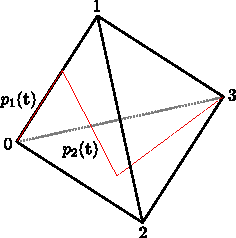
\includegraphics[scale=1]{aux/theta1.pdf}
	\caption{In red, the path $\theta_3(\bft) \in P(\gsimplex^3, v_0, v_3)$ associated to a $\bft \in \gcube^2$.}
	\label{f:theta1}
\end{figure}

A straightforward computation proves that the conditions in \cref{ss:adams maps} are satisfied by this collection.
A diagrammatical verification in low dimensions is provided in \cref{f:theta3}.

\begin{figure}[b]
	\centering
	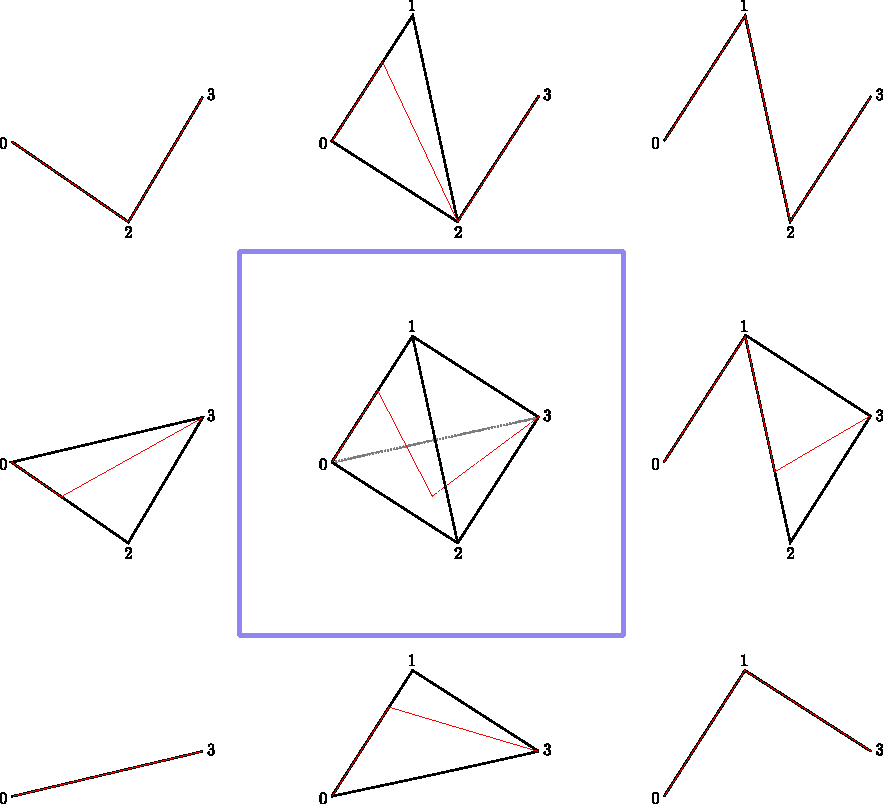
\includegraphics[scale=.5]{aux/theta3.pdf}
	\caption{The faces of the $2$-cube in blue, labeled by a red element in their corresponding family of paths.}
	\label{f:theta3}
\end{figure}

We can extend this collection $\{\theta_n \colon \gcube^{n-1} \to P(\gsimplex^n;v_0,v_n)\}$ to one of the form
\[
\set[\big]{\theta_{(n_1, \dots, n_k)} \colon \gcube^{n_1 + \dots + n_k-k} \to P(\gsimplex^{n_1} \vee \cdots \vee \gsimplex^{n_k})}
\]
where the \textit{topological necklace} $\gsimplex^{n_1} \vee \cdots \vee \gsimplex^{n_k}$ is obtained by identifying the last vertex of $\gsimplex^{n_i}$ with the first vertex of $\gsimplex^{n_{i+1}}$ for each $i = 1, \dots, k-1$ assuming each $n_i > 0$.
We do so by setting
\begin{multline*}
	\theta_{(n_1, \ldots, n_k)}(t_1, \ldots, t_{n_1+ \cdots + n_k-k}) \\ =
	\theta_{n_1}(t_1, \ldots, t_{n_1-1}) \cdot\ \dots\ \cdot \theta_{n_k}(t_{n_1+ \cdots n_{k-1}-k},\ldots,t_{n_1 + \cdots +n_k-k}).
\end{multline*}
Thus we can think of the topological necklace $\gsimplex^{n_1} \vee \cdots \vee \gsimplex^{n_k}$ as a space parameterizing a $(n_1+ \cdots + n_k-k)$-dimensional family of paths between the first and last vertices.
Please consult \cref{f:theta2} for an example illustrating this construction.

\begin{figure}
	\centering
	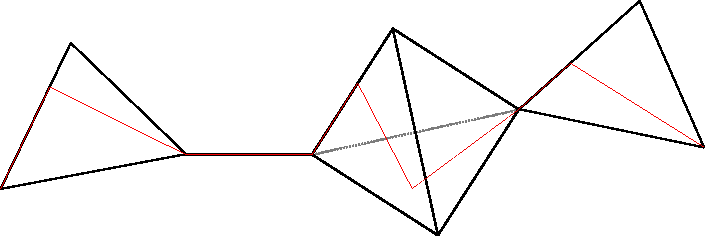
\includegraphics[scale=1]{aux/theta2.pdf}
	\caption{In red, the path $\theta_{(2,1,3,2)}(\bft)$ in $P(\gsimplex^2 \vee \gsimplex^1 \vee \gsimplex^3 \vee \gsimplex^2)$ associated to an element $\bft$ in $\gcube^{4}$.}
	\label{f:theta2}
\end{figure}

\subsection{Necklaces}

We now present a categorical viewpoint on the necklaces encountered in the previous subsection and their intimate relationship with Adams' cobar construction.
For any pointed space $(\fX,x)$, the underlying graded $\k$-module of $\cobar \sSchainsA(\fX,x)$ can be described as the graded $\k$-module freely generated by finite ordered sequences
\[
T = (\sigma_1, \dots, \sigma_k)
\]
of simplices $\sigma_i \in \sSing(\fX,x)$, with degree $\bars{T} = \bars{\sigma_1}+\dots+\bars{\sigma_k} - k$, modulo the sub $\k$-module generated by those sequences with at least one degenerate simplex.
The differential of $\cobar \sSchainsA(\fX,x)$ on a generator $T$ of degree $n$ is given by a signed sum of all generators $T'$ of degree $n-1$ that, in certain sense, fit inside $T$.
Furthermore, the monoid structure of $\cobar \sSchainsA(\fX,x)$ is induced by simply concatenating these ordered sequences of simplices.
This perspective suggests that $\cobar \sSchainsA(\fX,x)$ may be obtained by applying a normalized chains functor to certain cellular monoid, naturally associated to $(\fX,x)$, with cells labeled by finite ordered sequences of simplices in $\sSing(\fX,x)$.
A geometric construction reflecting this idea was described in \cite{baues1980geometry}.
We instead take a categorical approach and make this discussion precise through the framework of \textit{necklaces} and \textit{necklical sets} as we now discuss.

Consider the subcategory $\simplex_{*,*}$ of the simplex category $\simplex$ with the same objects and morphisms given by functors $f \colon [n] \to [m]$ satisfying $f(0) = 0$ and $f(n) = m$.
It is a strict monoidal category when equipped with the monoidal structure $[n] \ot [m] = [n+m]$, thought of as identifying the elements $n \in [n]$ and $0 \in [m]$, and unit given by $[0]$.
Heuristically, we may think of $\simplex_{*,*}$ as a category of models for cells parameterizing families of paths with fixed endpoints inside a simplex.

%In passing, we mention that this category is $\op$-dual to the augmented simplex category, a form of Joyal duality.
%do we need this?

The \textit{necklace category} $\Nec$ is obtained from $\simplex_{*,*}$ as follows.
Thinking of $\simplex_{*,*}$ as a monoid in $\Cat$, we first apply the bar construction to it and produce a simplicial object in $\Mon_{\Cat}$ which, after realization, defines the strict monoidal category $\Nec$.
We denote the monoidal structure by
\[
\vee \colon \Nec \times \Nec \to \Nec.
\]
We describe $(\Nec, \vee)$ in more explicit terms.
The objects of $\Nec$, called \textit{necklaces}, are freely generated by the objects of $\simplex_{*,*}$ through the monoidal structure $\vee$.
Namely, the set of objects of $\Nec$ is the set of monomials
\[
\big\{ [n_1] \vee \dots \vee[n_k] \mid n_i, k \in \N_{>0} \big\}
\]
together with $[0]$ serving as the monoidal unit.

The morphisms of $\Nec$ are generated through the monoidal structure by the following four types of morphisms for all $n \in\N_{>0}$
\begin{enumerate}
	\item $\partial^j \colon [n-1] \to [n]$ for $j = 1, \dots, n-1$,
	\item $\Delta_{[j], [n-j]} \colon [j] \vee [n-j] \to [n]$ for $j = 1, \dots, n-1$,
	\item $\xi^j \colon [n+1] \to [n]$ for $j = 0, \dots, n$ and $n>0$, and
	\item $\xi^0 \colon [1] \to [0]$.
\end{enumerate}
We may identify $\Nec$ with a full sub-category of the category of double pointed simplicial sets $\sSet_{*,*}$ as follows.
Consider the functor
\[
\mathcal{S} \colon \Nec \to \sSet_{*,*}
\]
induced by sending any necklace $T = [n_1] \vee \dots \vee[n_k]$ to the simplicial set
\[
\mathcal{S}(T) = \simplex^{n_1} \vee \dots \vee \simplex^{n_k},
\]
where the wedge symbol now means we identify the last vertex of $\simplex^{n_i}$ with the first vertex of $\simplex^{n_{i+1}}$ for $i = 1, \dots, k-1$ and the two base points are given by the first vertex of $\simplex^{n_1}$ and the last vertex of $\simplex^{n_k}$.
Then $\mathcal{S}$ is a fully faithful functor, so $\Nec$ may be identified with the full sub-category of $\sSet_{*,*}$ having as objects those double pointed simplicial sets of the form $\simplex^{n_1} \vee \dots \vee \simplex^{n_k}$.
The \textit{dimension} of a necklace $T = [n_1] \vee\dots\vee [n_k]$ is defined by $\dim(T) = n_1 + \dots + n_k-k$. Note there is a canonical homeomorphism \[\gsimplex^{n_1} \vee \cdots \vee \gsimplex^{n_k} \cong | \simplex^{n_1} \vee \cdots \vee \simplex^{n_k}|.\] 


The category of \textit{necklical sets} $\Fun(\Nec^{\op}, \Set)$ becomes a (non-symmetric) monoidal category with monoidal structure induced from $(\Nec, \vee)$.
We denote the monoidal category of necklical sets by $\nSet$.

\begin{remark*}
	The category of necklaces was introduced in \cite{dugger2011rigidification} to give an explicit description of the homotopy coherent nerve functor and its left adjoint.
\end{remark*}



\subsection{From necklaces to cubes}
In \cref{explicitchoice} we described an explicit way of decomposing a topological necklace $\gsimplex^{n_1} \vee \cdots \vee \gsimplex^{n_k}$ into a family of paths connecting the first and last vertices parameterized by an $(n_1 + \cdots + n_k-k)$-dimensional cube. This construction satisfies conditions (1), (2), and (3) in \cref{ss:adams maps}. In particular, conditions (2) and (3) may be interpreted as saying that each face in the codimension $1$ boundary of such a cube of paths is in one-to-one correspondence with codimension $1$ ``sub-necklaces" inside $\gsimplex^{n_1} \vee \cdots \vee \gsimplex^{n_k}$ connecting the first and last vertices. Furthermore, sub-necklaces in $\gsimplex^{n_1} \vee \cdots \vee \gsimplex^{n_k}$ are in one-to-one correspondence with the poset \[\{ J \subseteq \{0,\ldots, n_1+ \cdots + n_k-k\} | 0,n_1+ \cdots +n_k-k \in J \}\]
ordered by inclusion, which has a canonical cubical structure. We build upon this observation to describe a functorial relation between necklaces and cubes. This will be used to explain how Adams' map is induced by a deeper categorical construction.

We begin by defining a monoidal functor
\[
\cP \colon \Nec \to \cube
\]
as follows.
First define $\cP[0] = 2^0$.
On any other necklace $T \in \Nec$, define $\cP(T) = 2^{\dim(T)}$.
In order to define $\cP$ on morphisms, it is sufficient to consider the following cases.
\begin{enumerate}
	\item For any coface map $\partial^j \colon [n] \to [n+1]$ such that $0< j<{n+1}$, define $\cP(\partial^j) \colon 2^{n-1}\to 2^{n}$ to be the cubical coface functor $\cP(f)= \delta_0^{j}$.

	\item For any $\Delta_{[j], [n+1-j]} \colon [j] \vee [n+1-j] \to [n+1]$ such that $0<j<n+1$, define
	\[
	\cP(\Delta_{[j], [n+1-j]}) \colon 2^{n-1}\to 2^{n}
	\]
	to be the cubical coface functor $\cP(f)=\delta_1^{j}$.

	\item We now consider codegeneracy maps of the form $\xi^j \colon [n+1] \to [n]$ for $n>0$.
	If $j=0$ or $j=n$, define $\cP(f) \colon 2^n \to 2^{n-1}$ to be the cubical codegeneracy functor $\cP(s^j)= \varepsilon^{j}$.
	If $0<j<n$, define $\cP(s^j) \colon 2^n \to 2^{n-1}$ to be the cubical coconnection functor $\gamma^{j}$.

	\item For $\xi^0 \colon [1] \to [0]$ define $\cP(\xi^0) \colon 2^0 \to 2^0$ to be the identity functor.
\end{enumerate}

\begin{remark*}
	The functor $\cP$ is neither faithful or full.
	However, for any necklace $T' \in \Nec$ with $\dim(T')=n+1$ and any cubical coface functor $\delta_{\epsilon}^j \colon 2^n \to 2^{n+1}$ for $0 \leq j \leq n+1$, there exists an map $f \colon T \hookrightarrow T'$, where $T \in \Nec$ with $\dim(T)=n$ such that $\mathcal{S}(f) \colon \mathcal{S}(T) \hookrightarrow \mathcal{S}(T')$ is an injective morphism in $\Nec$ and $\cP(f) = \delta_{\epsilon}^j$.
\end{remark*}

The functor $\cP \colon \Nec \to \cube$ induces an adjunction between $\cSet$ and $\nSet$ with right and left adjoint functors given respectively by
\[
\cP^\ast \colon \cSet \to \nSet,
\qquad \text{and} \qquad
\cP_{!} \colon \nSet \to \cSet.
\]
Explicitly, for a cubical set $Y \colon \cube^\op \to \Set$,
\[
\cP^\ast(Y)= Y \circ \cP^\op,
\]
and for a necklical set $K \colon \Nec^\op \to \Set$,
\[
\cP_{!}(K) \ =
\colim_{\mathcal{Y}(T) \to K} \cP(T) \ \cong
\colim_{\mathcal{Y}(T) \to K} \cube^{\dim(T)}.
\]
Since $\cP$ is a monoidal, the functor $\cP_{!} \colon \nSet \to \cSet$ is monoidal as well.

\subsection{Cubical cobar construction}\label{ss:cubical cobar}

Using the framework of necklical sets, we may reinterpret Baues' geometric cobar construction \cite{baues1980geometry} as a functor
\[
\ncobar \colon \sSet^0 \to \Mon_{\nSet},
\]
which we now define.

For any reduced simplicial set $X$, we define a necklical set $\ncobar(X) \colon \Nec^\op \to \Set$ having as necklical cells all necklaces inside $X$; namely
\[
\ncobar(X) \, = \! \colim_{\mathcal{S}(T) \to X} \mathcal{Y}(T).
\]
The monoidal structure $\vee \colon \Nec \times \Nec \to \Nec$ given by concatenation of necklaces induces a natural product
\[
\ncobar(X) \ot \ncobar(X) \to \ncobar(X)
\]
making $\ncobar(X)$ into a monoid in $\nSet$.

We may now define the \textit{cubical cobar construction}
\[
\ccobar \colon \sSet^0 \to \Mon_{\cSet}
\]
as the composition
\[
\ccobar = \cP_! \, \circ \ncobar.
\]
Since $\cP_!$ is monoidal, $\ccobar(X)$ is a monoid in $\cSet$.

\begin{remark}
	This reinterpretation of Baues' construction in terms of cubical sets was also studied in \cite{rivera2018cubical}.
	In this reference, it is also proven that the composition of functor $\mathcal{T} \circ \ccobar$, where $\mathcal{T} \colon \Mon_{\cSet} \to \Mon_{\sSet}$ is the triangulation functor, coincides with the left adjoint of the homotopy coherent nerve functor restricted to $\sSet^0.$
\end{remark}

\subsection{Relation to the cobar construction}

We now relate the cubical cobar functor $\ccobar \colon \sSet^0 \to \Mon_{\cSet}$ to the cobar construction $\cobar \colon \coAlg^\ast \to \Mon_{\Ch}$ (\cref{ss:cobar construction}).

\begin{theorem}\label{t:ccobar and cobar}
	There is a natural isomorphisms of functors
	\[
	\cchains \ccobar \cong \cobar \schainsA \colon \sSet^0 \to \Mon_{\Ch}.
	\]
\end{theorem}

\begin{proof}
	Denote by $\iota_n \in (\cube^n)_n$ the top dimensional non-degenerate element of the standard $n$-cube $\cube^n$.
	Note that for a reduced simplicial set $X$, we may represent any non-degenerate $n$-cube $\alpha \in (\cP_!(\ncobar(X)))_n$ as a pair $\alpha = [\sigma \colon \mathcal{Y}(T) \to X, \iota_n]$ for some $T = [n_1] \vee \dots \vee [n_k] \in \Nec$ with $\dim(T) = n_1 + \dots + n_k - k = n$.

	To define a monoidal chain map
	\[
	\varphi_X \colon \cchains(\cP_!(\ncobar(X))) \xra{\cong} \cobar \schainsA(X)
	\]
	it suffices to define it on any generator of the form $\alpha=[\sigma \colon \simplex^{n+1} \to X, \iota_{n}]$, i.e., when $T$ is of the form $T = [n+1]$, for some $n \geq 0$.
	If $n = 0$ let $\varphi_X(\alpha)= [\overline{\sigma}] + 1_\k$, where $[\overline{\sigma}] \in \s{-1} \overline{ \schains(X)} \subset \cobar \schainsA(X)$ denotes the (length $1$) generator in the cobar construction of $\schains(X)$ determined by $\sigma \in X_{n+1}$ and $1_\k$ denotes the unit of the underlying ring $\k$.
	If $n > 0$, we let $\varphi_X(\alpha)=[\overline{\sigma}]$.
	A straightforward computation yields that this gives rise to a well defined isomorphism of algebras, which is compatible with the differentials, and natural with respect to maps of simplicial sets.
\end{proof}

A similar result to \cref{t:ccobar and cobar} was observed in the case of $1$-reduced simplicial sets in \cite[Section~3.5]{berger1995loops}.

\subsection{Factorization of Adams's map}\label{ss:factorization of adams}

Adams's comparison map can be factored as a composition
\begin{equation}\label{e:factorization of adams}
	\theta_\fX \colon \cobar \sSchainsA(\fX,x) \xrightarrow{\cong}
	\cchains \ccobar(\sSing(\fX,x)) \xrightarrow{\cchains(\Theta)}
	\cSchains(\loops_x \fX).
\end{equation}
The first map is the monoidal isomorphism induced by \cref{t:ccobar and cobar}.
The second map is given by applying chains $\cchains \colon \Mon_{\cSet} \to \Mon_{\Ch}$ to the map of monoidal cubical sets
\[
\Theta \colon \ccobar(\sSing(\fX,x)) \to \cSing(\loops_x \fX)
\]
determined through the monoid structure by sending an $n$-simplex $(\sigma \colon \gsimplex^n \to \fX)$ to the singular $(n-1)$-cube
\[
P(\sigma) \circ \theta_n \colon \gcube^{n-1} \to \loops_x \fX,
\]
where the maps $\theta_n \colon \gcube^{n-1} \to P(\gsimplex^n;0,n)$ are discussed in \cref{ss:adams maps}.

\subsection{A monoidal coalgebra structure on the cobar construction}

We follow \cite{baues1998hopf} to construct a coalgebra structure on $\cobar \sSchainsA(\fX,x)$, compatible with both the differential and monoid structure, such that Adams's map becomes a map of monoids in the category of coalgebras.

Recall the Serre coalgebra lift $\cchainsA \colon \cSet \to \coAlg$ of $\cchains \colon \cSet \to \Ch$, the unique monoidal functor defined by the coalgebra structure on $\chains(\cube^1)$.
Since $\cchainsA$ is monoidal and $\ccobar(\sSing(\fX,x))$ is a monoid, $\cchainsA(\ccobar(\sSing(\fX,x)))$ is a monoid in $\coAlg$.
Similarly, the lift $\cchainsA$ equips $\cSing(\loops_x \fX)$ with a natural monoidal coalgebra structure as well.
Consequently, the isomorphism in (\ref{e:factorization of adams}) endows $\cobar \sSchainsA(\fX,x)$ with a natural monoidal coalgebra structure making $\theta_\fX$ into natural map of monoidal coalgebras.

